110. \begin{figure}[ht!]
\center{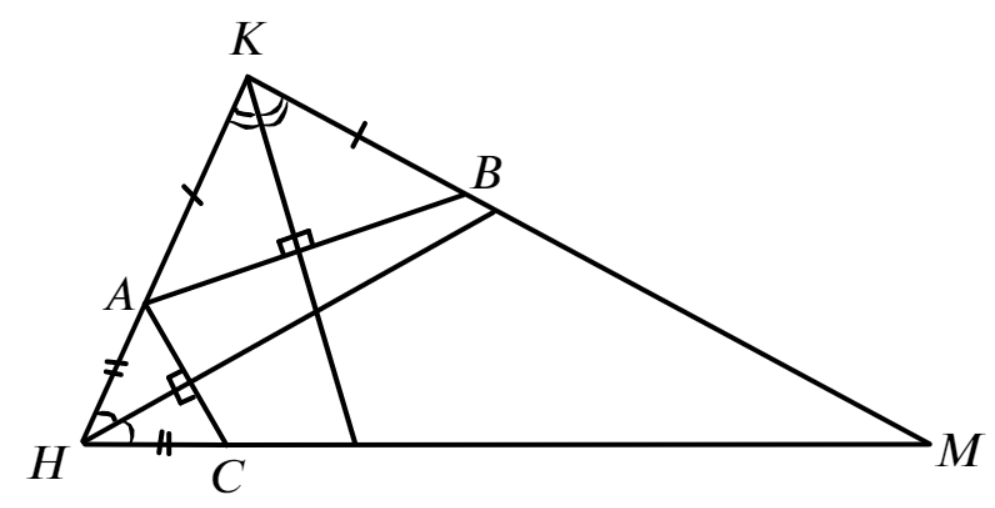
\includegraphics[scale=0.35]{g110.png}}
\end{figure}\\
В треугольниках $AHC$ и $AKB$ высота совпадает с биссектрисой, значит они равнобедренные. Введём обозначения $AH=HC=x,\ KA=KB=y,\ MC=z,\ MB=2z.$ Тогда получаем систему уравнений $\begin{cases} x+y=12,\\ x+z=7,\\ y+2z=17.\end{cases}$ Домножим второе уравнение на 2, сложим с первым и вычтем третье, получим $2x+2z+x+y-y-2z=12+14-17,\ 3x=9,\ x=3.$ Тогда $y=12-3=9$ и отношение равно $1:3.$
ewpage
oindent
